\subsection{Spatiotemporal Visualization}
\label{sec:spatiotemporal_visualization}

\begin{figure}[tb]
\centering
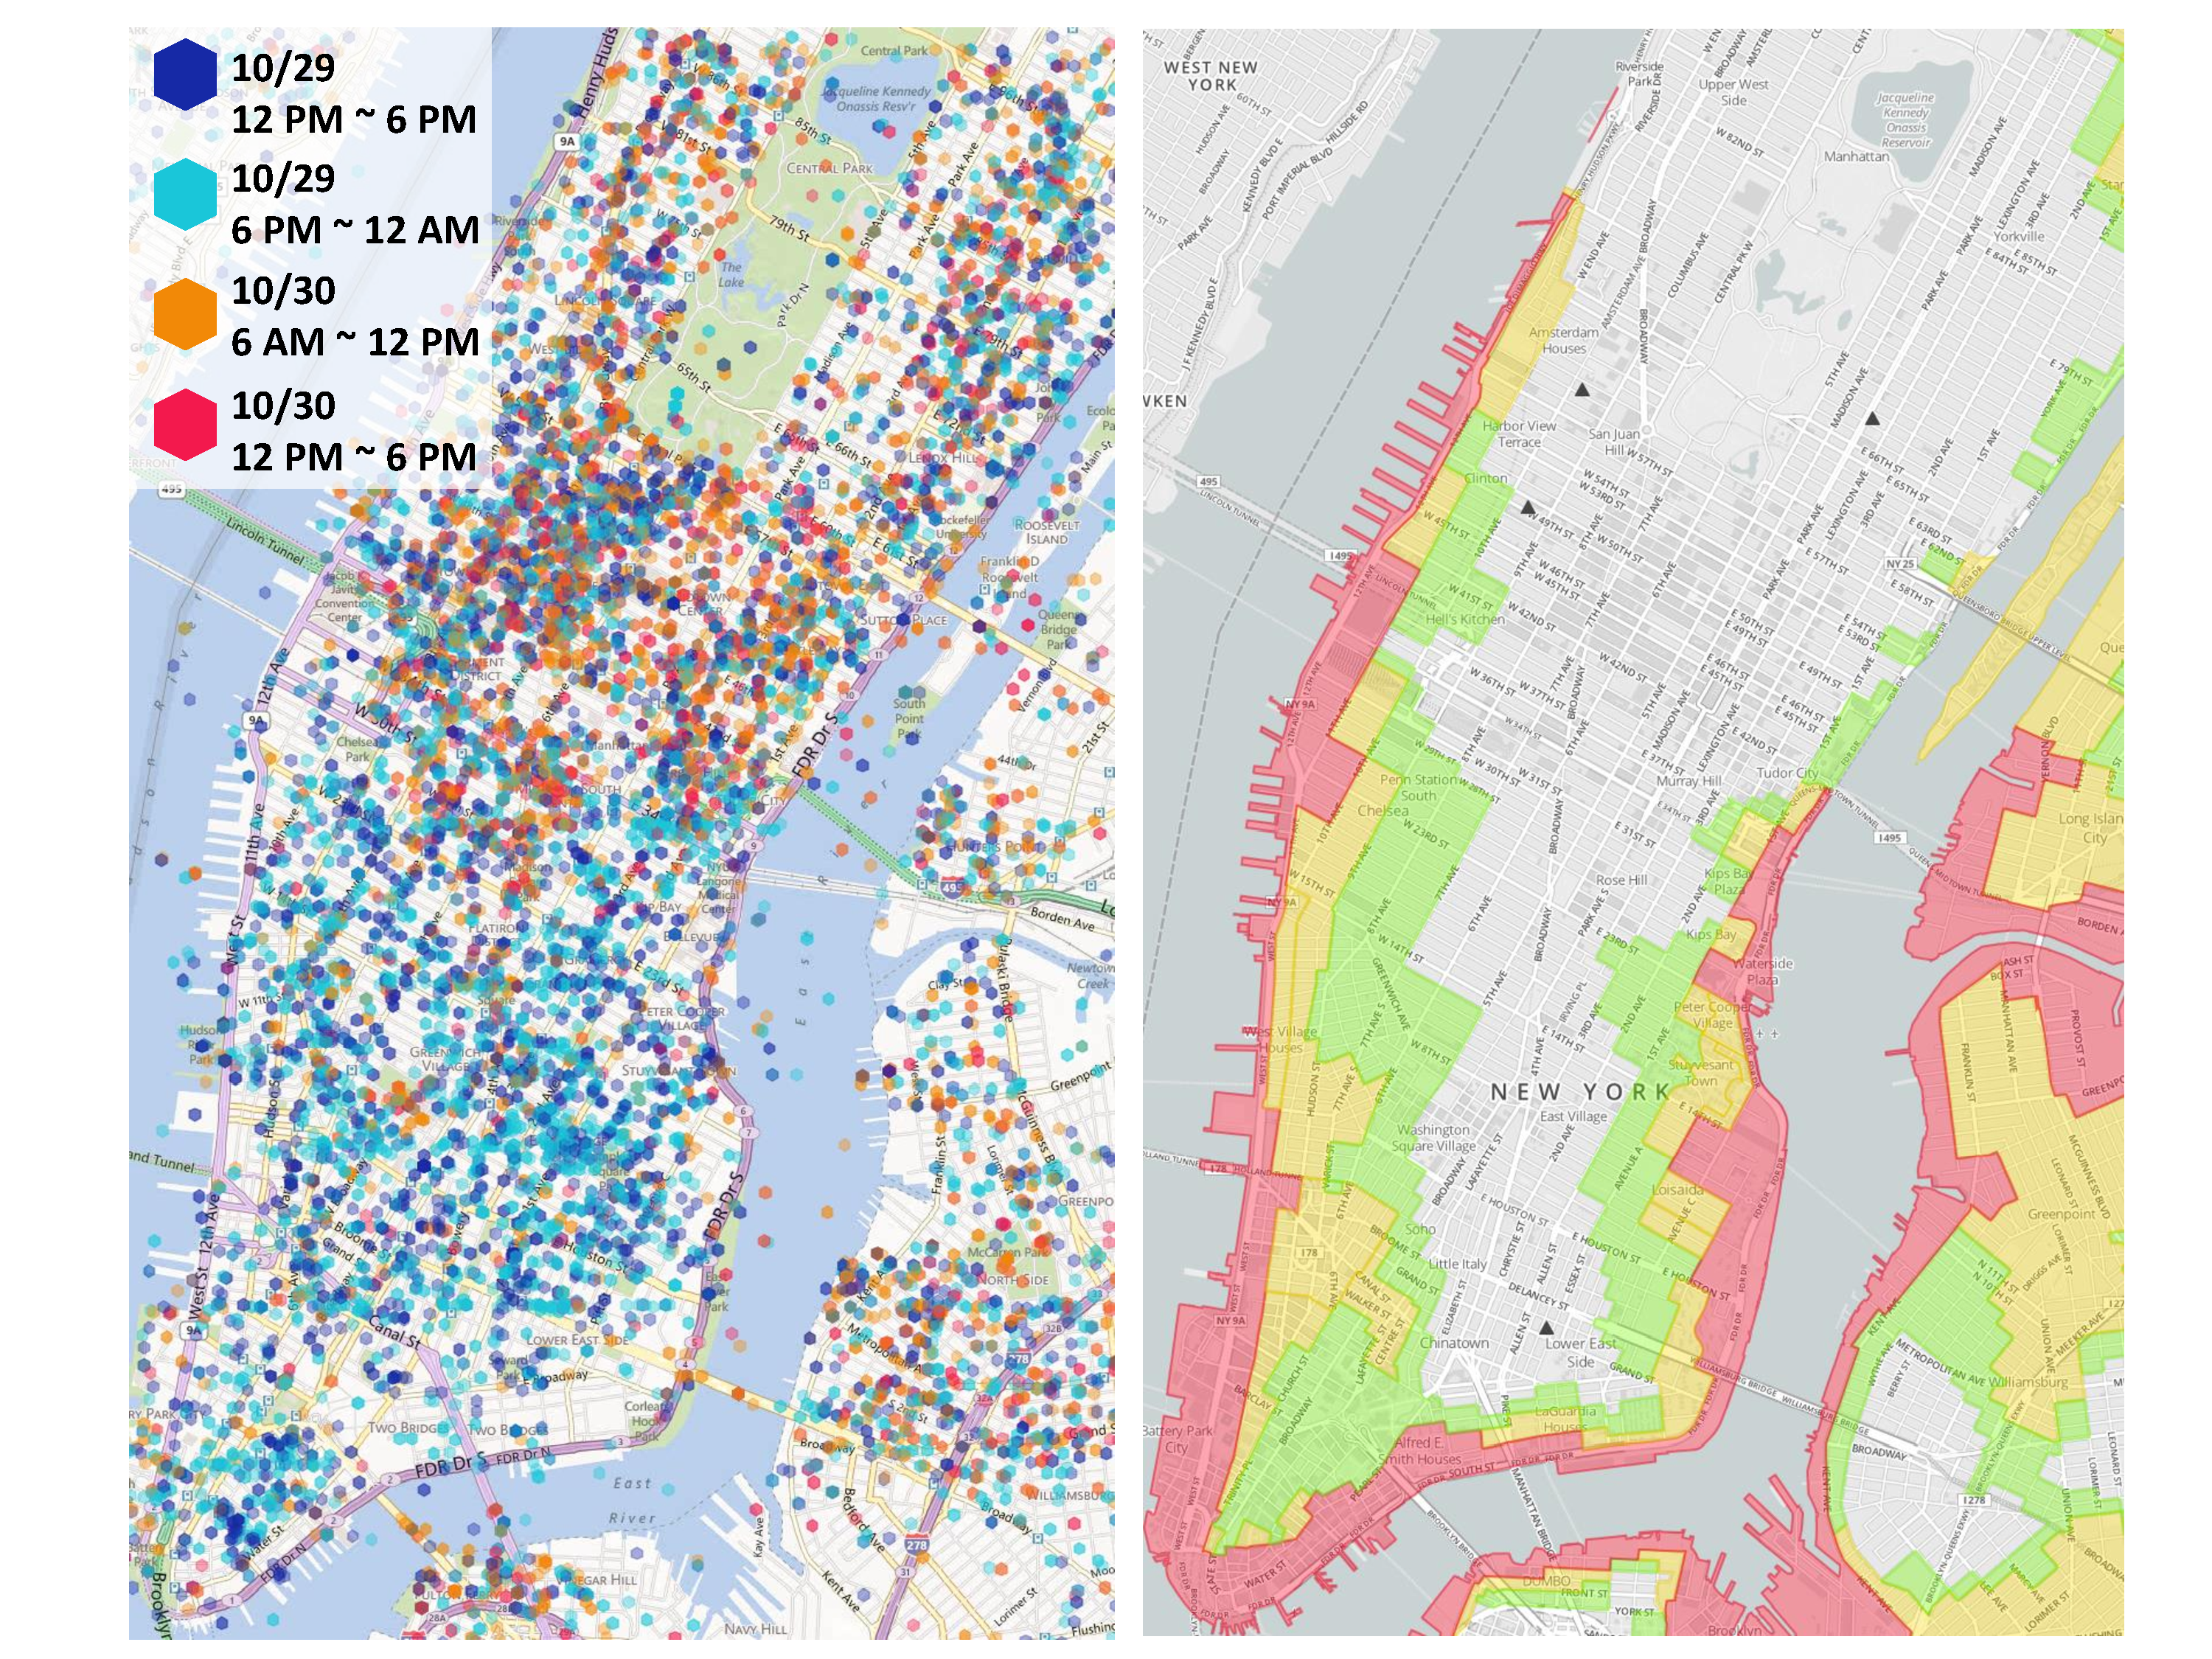
\includegraphics[width=1.0\linewidth]{spatiotemporal4}
\caption{Visualization for spatiotemporal social media data (Left).
A hexagon represents the spatial (position) and temporal (color) information of a Tweet.
Hurricane evacuation map~\cite{NYC:2012:HEM} (Right). Residents in Zone A (red) faced the highest risk of flooding, Zone B (yellow) and Zone C (green) are moderate and low respectively.}
\label{fig:spatiotemporal}
%\vspace{-0.8cm}
\end{figure}


There is abundant research published on the topic of spatiotemporal data visualization.
Still, exploration of time-referenced geographic data is still a challenging issue~\cite{Andrienko:2003:ESV}.
We introduce a modest visualization that enables analysts to analyze both aspects: space and time in a single view.
Each Tweet is independent and contains multiple properties, such as location, time, the number of re-Tweet, etc.
In this study, therefore, we utilize a glyph-based visualization to depict both location and time aspects of the independent data record using two visual features.
As shown in Figure~\ref{fig:spatiotemporal}~(Left), each hexagon corresponding to a Tweet represents the spatial and temporal information where the center of each hexagon is the location of each Tweet and the color represents its posting time.
In other words, space and time properties are encoded in a single visualization to harness the spatial analysis features of human visual perception~\cite{Treisman:1980:FIT}.
In Figure~\ref{fig:spatiotemporal}~(Left), the hexagons with blue~(12 PM $\sim$ 6 PM) or green~(6 PM $\sim$ 12 AM) ) color correspond to Tweets published on October 29th, 2012 and ones with orange or red color correspond to Tweets posted on the following day after the hurricane.
New York City announced the evacuation of Zone~A~(red color) in Figure~\ref{fig:spatiotemporal}~(Right); residents in Zone~A faced the highest risk of flooding, whereas, Zone~B~(yellow color) and Zone~C~(green color) are moderate and low respectively.
In the visual representation, analysts can indicate overall spatiotemporal patterns of people and their movements during the disaster event\textemdash many people still remained at home one day after the mandatory evacuation order, but most people left home on the following day as the hurricane damaged the city.